%-*-latex-*-
\sectionthree{Tree}
\begin{python0}
from solutions import *; clear()
\end{python0}

A tree is just a connected graph without cycles.
In this case, I'm talking about a tree as an undirected
graph.
You have to be careful, sometimes, a tree can also 
refer to a tree as a directed graph and acyclic.

Sometimes a special node is selected.
In this case, such a tree is sometimes called a rooted tree
(or a tree with a root).

Here's a tree (directed version):


\begin{center}
\begin{tikzpicture}[>=triangle 60,shorten >=0.5pt,node distance=2cm,auto,initial text=, double distance=2pt]
\node[state] (A) at (  3,  0) {$A$};
\node[state] (B) at (  6,  0) {$B$};
\node[state] (S) at (  0, -2) {$S$};
\node[state] (C) at (  3, -4) {$C$};

\path[->]
(A) edge [bend left=0,pos=0.5,above] node {} (B)
(A) edge [bend left=0,pos=0.5] node {} (C)
(S) edge [bend left=0,pos=0.5,above] node {} (A)
(S) edge [bend left=0,pos=0.5,above] node {} (C)

;
\end{tikzpicture}
\end{center}
    


\begin{myenum}

  \li
  $a$ is the \defone{root} of the tree.

  \li
  $a$ has 3 \defone{children}, i.e., $b,c,d$; 
  $a$ has a
  \sidebarskip{8pt}
  \defone{branching factor} 
  of 3.
  Sometimes, it's convenient to number the children.
  I'll call $b$ child $0$ of $a$; $d$ is child $2$ of $a$.

  \li
  $a$ is the \defone{parent} of $b$.

  \li
  $k$,$l$,$f$,$g$,$m$,$i$,$j$ are called
  \sidebarskip{-2pt}
  \defone{leaves}
  or
  \sidebarskip{12pt}\defone{non-internal} nodes because
  they don't have children.

  \li
  $a,b,c,d,e,h$ are called
  \sidebarskip{-2pt}
  \defone{non-leaf} nodes or 
  \sidebarskip{12pt}\defone{internal} nodes because 
  each have at least one child.

  \li
  $b$ has a \defone{depth} of $1$, i.e., 
  the length of the path from the root to $b$
  is 1. I will also say that $b$ is at level $1$.
  A root (see $a$ above) has depth 0.

  \li
  $b$ has a \defone{height} of $2$, i.e., 
  the length of the longest path from 
  $b$ to a leaf is 2.
  A leaf (see $k$ above) has height 0.

  \li
  The \defone{height} of a tree is the height of the root of the tree.
  The above tree has a height of 3.
  The height of an empty tree is -1.

  \li
  The root is at level 0. $b,c,d$ are at level 1.
  $e,f,g,h,i,j$ are at level 2. $k,l,m$ are at level 3.
  
  \li
  Two nodes $u$ and $v$ are \defone{siblings} if they have
  the same parent.
  For instance $b,c,d$ are siblings.
  
  \li
  $u$ has \defone{descendent} $v$ if there is a sequence of nodes 
  $u = v_0$, $v_1$, ..., $v_n = v$ where $v_i$ is the parent of $v_{i+1}$.
  $v$ is the \defone{ancestor} of $u$ if $u$ is a descendent of $v$.
  For instance in the above tree $b$ is an ancestor of $i$ and
  $i$ is a descendent of $l$.

\end{myenum}
Note that the above tree is a directed graph.
The following is also a tree (as in an \textit{undirected} tree).

%-*-latex-*-
{\footnotesize \begin{Verbatim}[frame=single,fontsize=\small]
[student@localhost discrete-probability] python tossfaircoin2.py
experiment 0 ... outcome: TAIL
experiment 1 ... outcome: TAIL
experiment 2 ... outcome: TAIL
experiment 3 ... outcome: TAIL
experiment 4 ... outcome: TAIL
experiment 5 ... outcome: TAIL
experiment 6 ... outcome: HEAD
experiment 7 ... outcome: TAIL
experiment 8 ... outcome: TAIL
experiment 9 ... outcome: TAIL
experiment 10 ... outcome: TAIL
experiment 11 ... outcome: HEAD
experiment 12 ... outcome: HEAD
experiment 13 ... outcome: TAIL
experiment 14 ... outcome: HEAD
experiment 15 ... outcome: TAIL
experiment 16 ... outcome: TAIL
experiment 17 ... outcome: HEAD
experiment 18 ... outcome: HEAD
experiment 19 ... outcome: TAIL
number of experiments: 20
number of heads: 6
number of tails: 14
probability of getting head: 0.3
probability of getting tail: 0.7
\end{Verbatim}
}


In the case of implementation, you can think of the directed version
as having pointers from a parent to the children.
In the case of the undirected version, you can think of
each edge as allowing you to go both up and down -- 
nodes having pointers going to their children or parent.
Of course exceptions being that roots have no parents and leaves have no
children.

For each node of a tree $T$, if you consider all the descendents of the node, 
you have a tree. This is called a \defone{subtree} of $T$.
For instance

\begin{console}
12094
\end{console}


is a subtree of 

\begin{center}
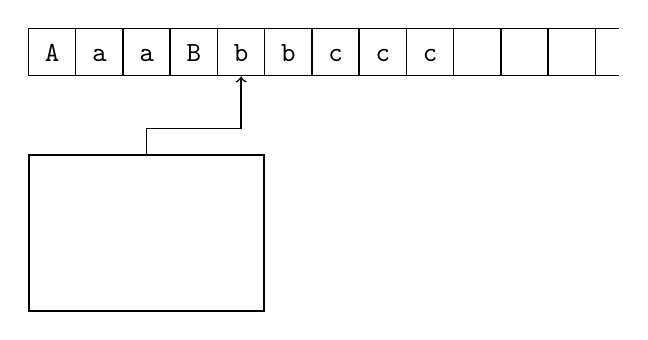
\begin{tikzpicture}

\draw (0.3, 0.3)
  node[draw, line width=0.02cm, , color=black,
       rounded corners=0cm, inner sep=0cm] {

\begin{minipage}[t][0.6cm]{0.6cm}
\mbox{}

\end{minipage}

};\draw (0.3, 0.3) node[color=black] {{\vphantom{AaaBbbccc$\BLANK$$\BLANK$$\BLANK$}\texttt{A}}};
\draw (0.8999999999999999, 0.3)
  node[draw, line width=0.02cm, , color=black,
       rounded corners=0cm, inner sep=0cm] {

\begin{minipage}[t][0.6cm]{0.6cm}
\mbox{}

\end{minipage}

};\draw (0.8999999999999999, 0.3) node[color=black] {{\vphantom{AaaBbbccc$\BLANK$$\BLANK$$\BLANK$}\texttt{a}}};
\draw (1.5, 0.3)
  node[draw, line width=0.02cm, , color=black,
       rounded corners=0cm, inner sep=0cm] {

\begin{minipage}[t][0.6cm]{0.6cm}
\mbox{}

\end{minipage}

};\draw (1.5, 0.3) node[color=black] {{\vphantom{AaaBbbccc$\BLANK$$\BLANK$$\BLANK$}\texttt{a}}};
\draw (2.0999999999999996, 0.3)
  node[draw, line width=0.02cm, , color=black,
       rounded corners=0cm, inner sep=0cm] {

\begin{minipage}[t][0.6cm]{0.6cm}
\mbox{}

\end{minipage}

};\draw (2.0999999999999996, 0.3) node[color=black] {{\vphantom{AaaBbbccc$\BLANK$$\BLANK$$\BLANK$}\texttt{B}}};
\draw (2.7, 0.3)
  node[draw, line width=0.02cm, , color=black,
       rounded corners=0cm, inner sep=0cm] {

\begin{minipage}[t][0.6cm]{0.6cm}
\mbox{}

\end{minipage}

};\draw (2.7, 0.3) node[color=black] {{\vphantom{AaaBbbccc$\BLANK$$\BLANK$$\BLANK$}\texttt{b}}};
\draw (3.3, 0.3)
  node[draw, line width=0.02cm, , color=black,
       rounded corners=0cm, inner sep=0cm] {

\begin{minipage}[t][0.6cm]{0.6cm}
\mbox{}

\end{minipage}

};\draw (3.3, 0.3) node[color=black] {{\vphantom{AaaBbbccc$\BLANK$$\BLANK$$\BLANK$}\texttt{b}}};
\draw (3.9000000000000004, 0.3)
  node[draw, line width=0.02cm, , color=black,
       rounded corners=0cm, inner sep=0cm] {

\begin{minipage}[t][0.6cm]{0.6cm}
\mbox{}

\end{minipage}

};\draw (3.9000000000000004, 0.3) node[color=black] {{\vphantom{AaaBbbccc$\BLANK$$\BLANK$$\BLANK$}\texttt{c}}};
\draw (4.5, 0.3)
  node[draw, line width=0.02cm, , color=black,
       rounded corners=0cm, inner sep=0cm] {

\begin{minipage}[t][0.6cm]{0.6cm}
\mbox{}

\end{minipage}

};\draw (4.5, 0.3) node[color=black] {{\vphantom{AaaBbbccc$\BLANK$$\BLANK$$\BLANK$}\texttt{c}}};
\draw (5.1, 0.3)
  node[draw, line width=0.02cm, , color=black,
       rounded corners=0cm, inner sep=0cm] {

\begin{minipage}[t][0.6cm]{0.6cm}
\mbox{}

\end{minipage}

};\draw (5.1, 0.3) node[color=black] {{\vphantom{AaaBbbccc$\BLANK$$\BLANK$$\BLANK$}\texttt{c}}};
\draw (5.699999999999999, 0.3)
  node[draw, line width=0.02cm, , color=black,
       rounded corners=0cm, inner sep=0cm] {

\begin{minipage}[t][0.6cm]{0.6cm}
\mbox{}

\end{minipage}

};\draw (5.699999999999999, 0.3) node[color=black] {{\vphantom{AaaBbbccc$\BLANK$$\BLANK$$\BLANK$}\texttt{$\BLANK$}}};
\draw (6.299999999999999, 0.3)
  node[draw, line width=0.02cm, , color=black,
       rounded corners=0cm, inner sep=0cm] {

\begin{minipage}[t][0.6cm]{0.6cm}
\mbox{}

\end{minipage}

};\draw (6.299999999999999, 0.3) node[color=black] {{\vphantom{AaaBbbccc$\BLANK$$\BLANK$$\BLANK$}\texttt{$\BLANK$}}};
\draw (6.899999999999999, 0.3)
  node[draw, line width=0.02cm, , color=black,
       rounded corners=0cm, inner sep=0cm] {

\begin{minipage}[t][0.6cm]{0.6cm}
\mbox{}

\end{minipage}

};\draw (6.899999999999999, 0.3) node[color=black] {{\vphantom{AaaBbbccc$\BLANK$$\BLANK$$\BLANK$}\texttt{$\BLANK$}}};\draw[line width=0.02cm,black] (7.1999999999999975,0.6) to  (7.499999999999998,0.6);
\draw[line width=0.02cm,black] (7.1999999999999975,0.0) to  (7.499999999999998,0.0);

\draw (1.5, -2.0)
  node[draw, line width=0.02cm, , color=black,
       rounded corners=0cm, inner sep=0cm] {

\begin{minipage}[t][1.98cm]{2.98cm}
\mbox{}

\end{minipage}

};\draw[line width=0.02cm,black,->] (1.5,-1) to  (1.5,-0.67) to  (2.7,-0.67) to  (2.7,-0.01);
\end{tikzpicture}

\end{center}



I will say that this is the subtree at $b$.

In the case of a node with two child, 
there are two subtrees, the subtree on the left is called the 
\defone{left subtree} and the one on the right is called the 
\defone{right subtree}.
(Duh.)
Look at the subtree at $b$:

%-*-latex-*-
\begin{Verbatim}[frame=single,fontsize=\small]
[student@localhost discrete-probability] python discrete-probrobability/game2.py
python: can't open file 'discrete-probrobability/game2.py': [Errno 2] No such fi
le or directory
\end{Verbatim}



The nodes $e,k,l$ form the left subtree of $b$
and the single node $f$ form the right subtree of $b$.


A tree is said to be \defone{$k$--ary} if every node has at most $k$ children;
that's the same as saying that every node has a maximum branching factor of
$k$.
In particular, a \defone{binary} tree is a tree with at most 2 children.


\begin{ex} 
  \label{ex:some-decision1}
  \tinysidebar{\debug{exercises/{empty0/question.tex}}}
  \solutionlink{sol:some-decision1}
  \qed
\end{ex} 
\begin{python0}
from solutions import *
add(label="ex:some-decision1",
    srcfilename='exercises/some-decision1/answer.tex') 
\end{python0}


We include the empty graph as a tree, except of course such trees
don't have roots.
Consider a $k$--ary tree $T$.
\begin{myenum}

\li $T$ is \defone{full} if every node has exactly $k$ children, except for 
the leaves, i.e., if every node has
either $k$ or $0$ children.
Here's a full binary tree:

\begin{center}
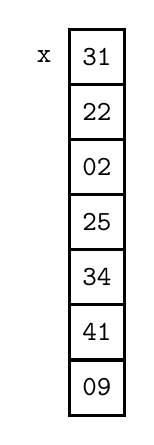
\begin{tikzpicture}

\draw (0.35, -0.35)
  node[draw, line width=0.04cm, , color=black,
       rounded corners=0cm, inner sep=0cm] {

\begin{minipage}[t][0.7cm]{0.7cm}
\mbox{}

\end{minipage}

};\draw (0.35, -0.35) node[color=black] {{\texttt{31}}};
\draw (0.35, -1.0499999999999998)
  node[draw, line width=0.04cm, , color=black,
       rounded corners=0cm, inner sep=0cm] {

\begin{minipage}[t][0.7cm]{0.7cm}
\mbox{}

\end{minipage}

};\draw (0.35, -1.0499999999999998) node[color=black] {{\texttt{22}}};
\draw (0.35, -1.7499999999999996)
  node[draw, line width=0.04cm, , color=black,
       rounded corners=0cm, inner sep=0cm] {

\begin{minipage}[t][0.7cm]{0.7cm}
\mbox{}

\end{minipage}

};\draw (0.35, -1.7499999999999996) node[color=black] {{\texttt{02}}};
\draw (0.35, -2.4499999999999997)
  node[draw, line width=0.04cm, , color=black,
       rounded corners=0cm, inner sep=0cm] {

\begin{minipage}[t][0.7cm]{0.7cm}
\mbox{}

\end{minipage}

};\draw (0.35, -2.4499999999999997) node[color=black] {{\texttt{25}}};
\draw (0.35, -3.15)
  node[draw, line width=0.04cm, , color=black,
       rounded corners=0cm, inner sep=0cm] {

\begin{minipage}[t][0.7cm]{0.7cm}
\mbox{}

\end{minipage}

};\draw (0.35, -3.15) node[color=black] {{\texttt{34}}};
\draw (0.35, -3.8499999999999996)
  node[draw, line width=0.04cm, , color=black,
       rounded corners=0cm, inner sep=0cm] {

\begin{minipage}[t][0.7cm]{0.7cm}
\mbox{}

\end{minipage}

};\draw (0.35, -3.8499999999999996) node[color=black] {{\texttt{41}}};
\draw (0.35, -4.550000000000001)
  node[draw, line width=0.04cm, , color=black,
       rounded corners=0cm, inner sep=0cm] {

\begin{minipage}[t][0.7cm]{0.7cm}
\mbox{}

\end{minipage}

};\draw (0.35, -4.550000000000001) node[color=black] {{\texttt{09}}};
\draw (-0.32, -0.35)
  node[draw=none, line width=0cm, , color=black,
       rounded corners=0cm, inner sep=0cm] {

\begin{minipage}[t][0.1cm]{0.1cm}
\mbox{}

\end{minipage}

};\draw (-0.32, -0.35) node[color=black] {\text{\texttt{x}}};
\end{tikzpicture}

\end{center}



Here's another:

\begin{console}[frame=single, , commandchars=~@$]
SLNode * p = phead;
while (p != NULL)
{
    std::cout << (*p) << std::endl;
    p = p->next();
}
\end{console}

and the output is this:
\begin{console}[frame=single,fontsize=\footnotesize]
[student@localhost linkedlist] g++ tmp12345678.cpp; ./a.out
<SLNode 0x7ffcf03deca0 key:2, next:0x7ffcf03decb0>
<SLNode 0x7ffcf03decb0 key:6, next:0x7ffcf03decc0>
<SLNode 0x7ffcf03decc0 key:4, next:0x7ffcf03decd0>
<SLNode 0x7ffcf03decd0 key:5, next:0>
\end{console}



\li $T$ is \defone{perfect} if $T$ is full and the leaves are 
at the same level.
Here's a perfect binary tree:


\begin{longtable}{|r||r|r|r|r|r|}
\hline 
         & $0$ & $1$ & $2$ & $3$ & $\ldots$ \\ \hline \hline 
$x_0$    & 5   & 0   & 0   & 0   & ...      \\ \hline 
$x_1$    & 1   & 4   & 1   & 5   & ...      \\ \hline 
$x_2$    &     &     &     &     &          \\ \hline 
$x_3$    &     &     &     &     &          \\ \hline 
$\ldots$ &     &     &     &     &          \\ \hline 
\end{longtable}
        

 
\li $T$ is \defone{complete} if it's \lq\lq almost full'' 
except that the last level 
might not have all the nodes. 
Here's a complete binary tree that is not full:

\begin{center}
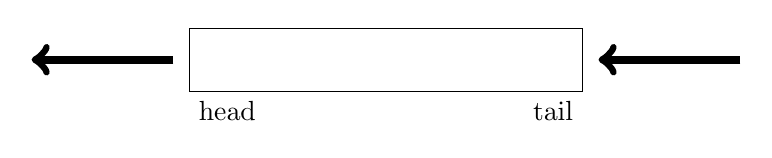
\begin{tikzpicture}

\draw (2.5, 0.4)
  node[draw, , , color=black,
       rounded corners=0cm, inner sep=0cm] {

\begin{minipage}[t][0.8cm]{5cm}
\mbox{}

\end{minipage}

};\draw[line width=0.1cm,black,->] (7,0.4) to  (5.2,0.4);
\draw[line width=0.1cm,black,->] (-0.2,0.4) to  (-2,0.4);

\node[anchor=north west] at (0,0)   {head};

\node[anchor=north east] at (5,0)   {tail};
\end{tikzpicture}

\end{center}


      
\li $T$ is \defone{balanced} if at each node,
every pair of children have heights differ by 0 or 1.
\end{myenum}

\begin{ex}
If $T$ is a balanced tree, does it mean that $T$ is complete?
If $T$ is complete, does it mean that $T$ is balanced?
\qed
\end{ex}

Let $T$ be a $k$--ary tree with height $h$ and the total 
number of nodes is $n$.
At level $\ell$,
there are at most $k^\ell$ nodes.
(Don't forget that the first level that contains only the root
is called level $0$.)
In particular for a binary tree, at level $\ell$, 
there are $2^\ell$ nodes.

Therefore if the height is $h$, $T$ can have at most
\[
k^0 + k^1 + \cdots + k^h = \frac{k^{h+1} - 1}{k-1}
\]
nodes.
(Remember your geometric sum formula?)
In particular, for a binary tree, $T$ can have at most
\[
2^{h+1} - 1
\]
nodes.
Since $T$ has $n$ nodes, we must have the following relation
between $n$ and $h$ for a $k$--ary tree:
\[
h + 1 \leq n \leq \frac{k^{h+1} - 1}{k-1}
\]
And for the case of binary tree, we have
\[
h + 1 \leq n \leq 2^{h+1}
\]

